\title{EE393 IEEE Paper}
\documentclass[journal,10pt]{IEEEtran}
\usepackage{cite}
\usepackage{amsmath} 
\usepackage{graphicx}
\usepackage{balance}

	\title{High Performance \\ Brushless DC Motor Drive}
	\author{Alan Lee,\textit{ Student}, Stuart Pollock, \textit{Student}, Daniel Murphy, \textit{Student} \\University of Washington \\ May 2016 
    \thanks{Funding provided by the College of Engineering and generous Electrical Engineering Alumni donations.}
    }
    \markboth{UW paper of stoof and tings} {}
\begin{document}
    \maketitle
    
\begin{abstract}
Brushless DC motors are electrically commutated synchronous which are powered by a DC source. The DC source is chopped up by a solid state inverter into an AC wave form, which is cycled through three phases of the motor’s stator to generate a cycling magnetic field to rotate a permanent or electromagnet. Brushless DC motors overcome many of the limitations brushed DC motors have, such as being quieter, undergoing less mechanical wear (lasting longer), running cooler, and having a higher efficiency. This report summarizes the design of a high performance electric drive for a Brushless DC motor. The drive features smooth acceleration, open-loop speed control, overcurrent and overvoltage protection, and regenerative braking. It accomplishes these features primarily with a microprocessor, inverter bridge, and gate driver.
\end{abstract}

\begin{IEEEkeywords}
DC machines, variable speed drive, inverters, microcontrollers
\end{IEEEkeywords}

\section{Introduction}
\IEEEPARstart{T}{he} purpose of this project is to create a high-performance brushless DC (BLDC) motor drive. This paper will step through the design process, and discuss difficulties encountered and conclusions reached. A motor controller or drive is what governs the operation of an electric motor. The rise of brushless DC motors, due to them lasting longer, running quieter, and operating more efficiently has lead to an increased need for engineering electric drives. This is opposed to a brushed motor which is simply given input voltage and commutated mechanically, which is loud and has a shorter lifespan. An intelligent motor controller uses a microprocessor to control the power electronics in an electric motor, which gives the drive better efficiency and higher performance. 

The goals of the project included designing a drive that will run with up to 48 $V_{dc}$ from a single power source, the maximum phase current cannot exceed 10 A, it will have bi-directional control, accelerate in 500 ms or less, regenerative braking to decelerate the motor in 500 ms or less, open-loop speed control, and over-voltage protection. 


\section{Method}
	An Arduino processor functioned as the rotary encoder, MOSFET signal generator, user input controller, and triggered overvoltage and overcurrent protection signals. For the encoding process, hall sensors on the motor’s stator trigger high and low signals according to the position of the rotor. These signals are then read by the ardiuno and processed to enforce the commutation pattern for the three-phase inverter bridge. The inverter bridge is made up of 6 IRF540 MOSFETs, the IRF540 are rated for 28 amps and is designed for high speed switching \cite{irf}. The gate signals at each MOSFET is feed by an HIP4086 bridge driver integrated circuit. The HIP4086 integrated circuit was selected as a bootstrap MOSFET gate driver to overcome the high-side MOSFET switching problem present in each phase of the inverter bridge \cite{hip}. A LM2596HV buck converter takes the supply voltage down to 12V to power the Arduino and HIP4086, and a linear voltage regulator is used to drop 12V to 5V to power op amp circuitry, hall sensors, and user input related components. A current sense resistor feeding an operational amplifier circuit was used for over-current protection, and a voltage divider was used for over-voltage sensing and protection The generalized circuit can be seen below in Figure 1.

\begin{figure}[h]
\centering
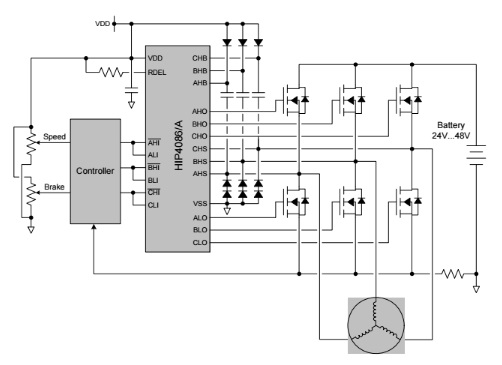
\includegraphics[scale =0.5]{hip.jpg}
\caption{Simplified motor drive circuit from \cite{hip}}

\end{figure}

    
\section{Results}
	The resulting circuit is able to operate with input voltages ranging from 12-48 volts.  With an input voltage at 48 volts the motor was able to accelerate up to full speed within 100 ms and regenerative breaking is implemented that can stop the motor within 80 ms. The circuit includes a start and stop button that allows an operator to control when the motor will be spinning. The operator is also able to control the speed and direction of the motor through the use of a potentiometer and switch respectively. 
\newpage
\balance
\section{discussion}
	Ultimately this brushless DC motor drive meets all the required specifications, however many improvements can be made as future work. The current design fails to close a current loop or speed loop, which reduced the circuit's ability to maintain a constant rotor speed. The regenerative braking feature isn't very robust and needs improvements, better filtering could be deployed to clean the control signals of any parasitic noise. The current limiter circuit could be redesigned for better delay times and to have a more robust hysteresis.
\vspace{0.5cm}

\bibliographystyle{IEEEtran}
\bibliography{biblo}



%need intro, methods, results, discussion, NO conclusion
\end{document}